% ----------------------------------------------------------------
% AMS-LaTeX Paper ************************************************
% **** -----------------------------------------------------------
\documentclass[oneside]{amsart}
\usepackage{graphicx}
\usepackage{color}
\usepackage[letterpaper]{geometry}
\usepackage[colorlinks=false,
            pdfborder={0 0 0},
            pdftitle={CSC488 A2},
            pdfauthor={Daniel Bloemendal},
            pdfsubject={CSC488},
            pdfstartview=FitH,
            pdfmenubar=false,
            pdfdisplaydoctitle=true,
            bookmarks=false]{hyperref}
\usepackage{subcaption}
\usepackage{mathtools}
\usepackage{listings}
\usepackage[table]{xcolor}
% ----------------------------------------------------------------
\vfuzz2pt % Don't report over-full v-boxes if over-edge is small
\hfuzz2pt % Don't report over-full h-boxes if over-edge is small
% THEOREMS -------------------------------------------------------
\newtheorem{thm}{Theorem}[section]
\newtheorem{cor}[thm]{Corollary}
\newtheorem{lem}[thm]{Lemma}
\newtheorem{prop}[thm]{Proposition}
\theoremstyle{definition}
\newtheorem{defn}[thm]{Definition}
\theoremstyle{remark}
\newtheorem{rem}[thm]{Remark}
\numberwithin{equation}{section}
% MATH -----------------------------------------------------------
\newcommand{\norm}[1]{\left\Vert#1\right\Vert}
\newcommand{\abs}[1]{\left\vert#1\right\vert}
\newcommand{\set}[1]{\left\{#1\right\}}
\newcommand{\Real}{\mathbb R}
\newcommand{\eps}{\varepsilon}
\newcommand{\To}{\longrightarrow}
\newcommand{\BX}{\mathbf{B}(X)}
\newcommand{\A}{\mathcal{A}}
\newcommand{\e}{\mathrm{e}}
\newcommand{\AND}{\wedge}
\newcommand{\OR}{\vee}
\newcommand{\NOT}{\neg}
\newcommand{\IMPLIES}{\to}
\newcommand{\TRUE}{\top}
\newcommand{\FALSE}{\bot}
\newcommand{\EQUALS}{\equiv}
\DeclareMathOperator{\sech}{sech}
\newcolumntype{B}{>{\columncolor{black}\color{white}}c}
% ----------------------------------------------------------------
\lstset {
    basicstyle=\fontsize{8}{11}\selectfont\ttfamily,
    frame=lines,
}
% ----------------------------------------------------------------

\begin{document}

\title[CSC488 A2]{CSC488\\ASSIGNMENT 2\\Grammar Design}
\author{Daniel Bloemendal}

% ----------------------------------------------------------------
\begin{titlepage}
\maketitle
\thispagestyle{empty}
\tableofcontents
\end{titlepage}
% ----------------------------------------------------------------

\section{Overview}
We began by translating the production rules in the reference grammar into Java CUP syntax. However,
the reference grammar is certainly not LALR. Furthermore, the reference grammar does not observe any
of the operator precedence rules described in the language documentation. So the next goal was to
begin transforming the production rules into LALR friendly rules, observing precedence in
expressions. The challenges encountered during this transformation will be outlined below.

\section{Shift/Reduce conflicts}
The reference grammar uses the following style to accept lists. It is used for instance to recognize
lists of statements or declarations.
\begin{lstlisting}
statement
    ::= ...
    |   ...
    |   statement statement
    ;
\end{lstlisting}
Unfortunately with LALR parsers, as soon as a statement is shifted on to the stack, there are two
valid actions. The statement on stack can be reduced to the ``statement'' non-terminal, or an
additional statement can be shifted on to the stack to satisfy the alternative
\begin{lstlisting}
    |   statement statement
\end{lstlisting}
The solution was to add explicit list production rules as follows.
\begin{lstlisting}
statement_list
    ::= statement_list statement
    |   statement
    ;
\end{lstlisting}
This resolves the issue as a reduction to ``statement\_list'' is only possible if there are no
remaining statements left to shift on to the stack. This transformation was applied for statements,
declarations and other such lists.

\newpage

\section{Reduce/Reduce conflicts}
Another problem encountered during the process of transforming the grammar was an ambiguity when it
came to variables and parameters. According to the reference grammar both a ``variablename'' and
and ``parametername'' can be reduced to a ``variable''. However, this is ambiguous as both
``variablename'' and ``parametername'' reduce from ``IDENT''. So in the case of ``variable'' if
an ``IDENT'' is shifted on to the stack there is more than one valid reduction. It can be reduced to
``variablename'' or ``parametername''. This is a reduce/reduce conflict.

\begin{lstlisting}
variable
    ::= variablename
    |   parametername
    |   variablename L_SQUARE expression R_SQUARE
    |   variablename L_SQUARE expression COMMA expression R_SQUARE
    ;

variablename  ::= IDENT;
parametername ::= IDENT;
\end{lstlisting}


\lstset{numbers=left}
\section{Expressions}
\subsection{Design}
The expression rules were built as a set of left recursive productions obeying the precedence rules
set out in the reference grammar documentation. When viewing an expression as a tree, it is easy to
see that the higher the precedence of an operation the closer it is to the bottom, or the leaves of
the tree.

%<TpX v="5" TeXFormat="none" ArrowsSize="0.7" StarsSize="1" DefaultFontHeight="5" DefaultSymbolSize="30" ApproximationPrecision="0.01" PicScale="1" Border="2" BitmapRes="20000" HatchingStep="2" DottedSize="0.5" DashSize="1" LineWidth="0.3">
%  <text x="43.7" y="97.2" t="+" tex="$+$" h="5"/>
%  <line x1="44" y1="96" x2="30" y2="90"/>
%  <line x1="60" y1="90" x2="47" y2="96"/>
%  <text x="23" y="85" t="x_1 * x_2" tex="$x_1* x_2$" h="5"/>
%  <text x="53.4" y="85" t="y_1 * y_2" tex="$y_1 * y_2$" h="5"/>
%</TpX>
\begin{figure}[h]
\centering
\ifpdf
  \caption{Expression: $x_1*x_2 + y_1*y_2$}
  \setlength{\unitlength}{1bp}
  \begin{picture}(154.20, 60.09)(0,0)
  \put(0,0){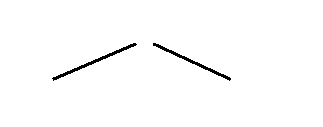
\includegraphics{expression.pdf}}
  \put(64.35,43.31){\fontsize{14.23}{17.07}\selectfont $+$}
  \put(5.67,8.73){\fontsize{14.23}{17.07}\selectfont $x_1* x_2$}
  \put(91.84,8.73){\fontsize{14.23}{17.07}\selectfont $y_1 * y_2$}
  \end{picture}
\else
\fi
\label{fig:expression}
\end{figure}


To illustrate how the expression productions were designed, we will explore a simplified grammar
involving only addition and multiplication. As in the reference grammar, addition has lower
precedence than multiplication. As seen in figure \ref{fig:expression}, the higher precedence
multiplication operations are at the leaves of the tree. The production rules can be constructed
to reflect this tree like structure of expressions.

\begin{lstlisting}
expressions
    ::= add_expr
    ;

add_expr
    ::= add_expr PLUS mul_expr
    |   mul_expr
    ;

mul_expr
    ::= mul_expr TIMES terminal
    |   terminal
    ;
\end{lstlisting}

Working from the top down, in our simplified grammar the root of an expression begins at an addition
expression, as seen in line 2. This reflects the fact that addition has the lowest precedence. The
addition production then eats up as many terms as exist in the input sum. This is found in line 6 of
the simplified grammar. When no terms are left in the sum ``add\_expr'' falls through to ``mul\_expr''
as seen in line 7 of the simplified grammar. If there is only one term, where no ``+'' operator 
exists in the expression, ``add\_expr'' immediately falls through to ``mul\_expr''. The  ``mul\_expr''
eats up all product operations and ends when there are none left. At the end only terminals remain
and the process is complete.

It should be noted, that we explored the grammar from the top down. The LALR parser of course works
from the bottom up. However, it is simpler to describe the design of the grammar working from the
top down. The final product is a slightly more complicated application of concepts in the simplified
grammar.

\lstset {
    basicstyle=\fontsize{8}{11}\selectfont\ttfamily,
    frame=none,
    numbers=none
}

\subsection{Difficulties}
While designing test cases we encountered a string that belongs to the reference language but is
not recognized by our parser.

\begin{lstlisting}
    b := 1 * not false
\end{lstlisting}

While the string is not semantically valid due to the type mismatch, where a boolean is one of the
operands of a numeric operator, it is a valid string in the reference language. The expression
productions rules were designed to obey operator precedence rules. The way the ``not'' rule was
setup was to expect a predicate expression after a list of ``not'' terminals. While this is
appropriate for practical purposes as it will accept all semantically valid expressions we have
tested, it unfortunately will not recognize all syntactically valid expressions. We decided not to
solve this problem as our only solutions increased grammar complexity for no practical gain.

% ----------------------------------------------------------------
\end{document}
% ----------------------------------------------------------------
